\newpage
\clearpage

% Mock Exam Part 1

\subsection{Exercise 1: Running Time}

\subsubsection{Example 1}
1. (6P) Write the following Theta-classes in non-decreasing order from left to right (i.e., smallest on the left):

$\Theta(n^2), \Theta(e^{\log_2 n}), \Theta(\sin n), \Theta(\ln^2 n), \Theta(\log_2 n), \Theta(n^3 + \ln(n^2)), \Theta(e^{n^2}), \Theta(e^{\ln(n^4)})$

Solution: Understand growth rates: $\sin n$ is slowest, followed by logarithmic, polynomial, and exponential. Use limits to compare and order.

2. (3P) We consider a recursive algorithm that involves an input with $n$ objects and having running time $T(n) = 4 \cdot T\left(\frac{n}{2}\right) + n^2$. Determine the running Theta class of the algorithm.

Solution: Identify recurrence: $T(n) = a \cdot T\left(\frac{n}{b}\right) + f(n)$. Apply Master Theorem: Compare $f(n)$ with $n^{\log_b a}$ and determine the case.

3. (3P) We consider a recursive algorithm that involves an input with $n$ objects and having running time $T(n) = 4 \cdot T(n/2) + n$. Determine the running Theta class of the algorithm.

Solution: Apply Master Theorem: Use Case 1 for $f(n) = O(n^{\log_b a - \epsilon})$.

4. (3P) We consider a recursive algorithm that involves an input with $n$ objects and having running time $T(n) = 4 \cdot T(n/2) + n^3$. Determine the running Theta class of the algorithm.

Solution: Apply Master Theorem: Use Case 3 for $f(n) = \Omega(n^{\log_b a + \epsilon})$.

\subsubsection{Solution:}
1. $\Theta(\sin n), \Theta(\log_2 n), \Theta(\ln^2 n), \Theta(n^2), \Theta(e^{\log_2 n}), \Theta(n^3 + \ln(n^2)), \Theta(e^{\ln(n^4)}), \Theta(e^{n^2})$

2. Case 2 Master theorem. $\Theta(n^2 \ln n)$.

3. Case 1 Master theorem. $\Theta(n^2)$.

4. Case 3 Master theorem. $\Theta(n^3)$. (In all three cases, 1p corrected answer 2p correct justification)

\subsubsection{Example 2}
1. (4P) Write in increasing order from left to right the following list of Theta classes. When two classes are equal, make it clear.

$\Theta(n^{4/5}), \Theta(100n), \Theta(n \log_4 n), \Theta(n^{3/2}), \Theta(n^{\sqrt{n}}), \Theta(e^{\sqrt{2} \cdot n}), \Theta(e^n), \Theta(n!)$

Solution: Understand growth rates: Familiarize yourself with common functions like polynomials, logarithms, exponentials, and factorials. Use limits to compare and order.

2. (2P) Give two functions $f(n)$ and $g(n)$ such that

$\Theta(f(n) + g(n)) \neq \Theta(f(n))$ and $\Theta(f(n) + g(n)) \neq \Theta(g(n))$

Solution: Choose functions with different growth rates.

\subsubsection{Solution:}
$\Theta(n^{4/5}), \Theta(100n), \Theta(n \log_4 n), \Theta(n^{\sqrt{n}}), \Theta(n^{3/2}) = \Theta(n^{\sqrt{n}}), \Theta(e^n), \Theta(e^{\sqrt{2} \cdot n}), \Theta(n!)$

$f(n) = n$ and $g(n) = -n + 1$

\subsection{Exercise 2: Pseudocode Examples}

\subsubsection{Example 1: Pseudocode}

1. (6P) Write a pseudocode, which takes the input $A = \{a_1,a_2,\ldots,a_n\}$ and gives you as output $B = \{a_n,\ldots,a_2,a_1\}$ (i.e. same entries as in $A$ but, in the reversed order).

Solution approach:
- Use array indexing to swap elements
- Only need to iterate through half the array (why? because each swap handles two positions)
- Track running time: each operation is constant time, done $n/2$ times

\begin{algorithm}
\begin{algorithmic}[1]
\Procedure{ReverseArray}{$A$}
\For{$i = 1$ to $\lfloor n/2 \rfloor$}
    \State exchange $A[i]$ with $A[n-i+1]$
\EndFor
\State \Return $A$
\EndProcedure
\end{algorithmic}
\end{algorithm}

Running time: $\Theta(n)$ because we perform $n/2$ constant-time operations.

2. (9P) Let $S$ be a set with $n$ integers, randomly ordered and not necessarily distinct. Let $m$ be an integer. Write a pseudocode, which tests whether there are two elements $a,b \in S$ with $a + b = m$ (a and b may be the same number).

Solution approach:
- Naive solution: Check all pairs with nested loops = $O(n^2)$
- Better solution: Sort first, then use two pointers = $O(n \log n)$
- Best solution: Single pass with smart pointer movement = $O(n)$

Naive solution (for understanding):
\begin{algorithm}
\begin{algorithmic}[1]
\Procedure{SumTest}{$S,m$}
\For{$i = 1$ to $n-1$}
    \For{$j = i+1$ to $n$}
        \If{$S[i] + S[j] = m$}
            \State \Return true
        \EndIf
    \EndFor
\EndFor
\State \Return false
\EndProcedure
\end{algorithmic}
\end{algorithm}

Optimized solution:
\begin{algorithm}
\begin{algorithmic}[1]
\Procedure{SumTestBest}{$S,m$}
\State $i \gets 1$, $j \gets n$
\While{$i < j$}
    \If{$S[i] + S[j] = m$}
        \State \Return true
    \ElsIf{$S[i] + S[j] < m$}
        \State $i \gets i+1$
    \Else
        \State $j \gets j-1$
    \EndIf
\EndWhile
\State \Return false
\EndProcedure
\end{algorithmic}
\end{algorithm}

Key insights for optimization:
- Avoid checking all pairs
- Use array properties to skip unnecessary checks
- Think about how to move pointers based on sum comparison with target
- Running time improves from $O(n^2)$ to $O(n)$

\subsection{Exercise 3: Sweep Line Algorithm}

\subsubsection{Example 1: ANYSEGMENTINTERSECT}

Given the algorithm ANYSEGMENTINTERSECT and line segments on an (x,y)-plane, determine the sweep lines and partial orders.

Solution approach:
1. Understand the algorithm:
   - Sorts endpoints from left to right
   - Maintains partial order of segments crossing sweep line
   - Checks for intersections at each event point

2. Steps to solve:
   a) First, identify all endpoints (left and right) of segments
   b) Sort them from left to right
   c) For each vertical sweep line at these points:
      - Draw the vertical line
      - List segments crossing this line from bottom to top
      - Check for intersections between adjacent segments

3. Key points to remember:
   - Left endpoint: INSERT segment into order
   - Right endpoint: DELETE segment from order
   - Check ABOVE and BELOW neighbors for intersections
   - Stop when intersection found

4. Example solution format:
   Sweep line at x = -2:
   Segments (bottom to top): a, f
   
   Sweep line at x = -1:
   Segments: a, e, f, b
   
   Sweep line at x = 0:
   Segments: c, e, f, b

Running time analysis:
- Sorting endpoints: $O(n \log n)$
- Each endpoint processed once: $O(n)$
- Total: $O(n \log n)$

Common mistakes to avoid:
- Don't forget to order segments from bottom to top
- Check both ABOVE and BELOW at insertion
- List ALL segments crossing each sweep line

\subsection{Exercise 4: Points on the Plane}

\subsubsection{Example 1: Points on the Plane}

1. (9P) Check for collinear points in 2D plane:

Solution steps:
a) For each point $p_0$ as center:
   - Calculate angles between $\overline{p_0p_1}$ and all other segments $\overline{p_0p_j}$
   - Use DIRECTION($p_0$, $p_i$, $p_j$) = cross product $(p_1 - p_0) \times (p_j - p_0)$
   - Calculate angle: $\alpha_j = \sin^{-1}\left(\frac{\text{cross product}}{||p_1-p_0|| \cdot ||p_j-p_0||}\right)$

b) For each center point:
   - Sort angles using merge sort: $O(n \log n)$
   - Use SUMTESTBEST to find angles with 0 or $\pi$ difference: $O(n)$
   - Three points collinear if difference is 0 or $\pi$

Total running time: $O(n^2 \log n)$ because:
- Repeat for each point: $O(n)$
- For each center: $O(n \log n)$ for sorting + $O(n)$ for checking
- Final complexity: $n \cdot O(n \log n) = O(n^2 \log n)$

2. (6P) BUILDKDTREE construction:

Steps to construct KD-Tree:
a) Start with depth 0 (vertical split)
   - Find median x-coordinate
   - Split points into left/right sets

b) At depth 1 (horizontal split):
   - Find median y-coordinate in each subset
   - Split into top/bottom sets

c) Continue alternating between:
   - Even depth: vertical splits (x-coordinate)
   - Odd depth: horizontal splits (y-coordinate)

Example tree structure:
\begin{algorithm}
\begin{algorithmic}[1]
\State At root (depth 0): vertical split
\State \quad Left child: points left of median
\State \quad Right child: points right of median
\State At depth 1: horizontal splits
\State \quad Top/bottom division for each subset
\end{algorithmic}
\end{algorithm}

Key insights:
- Alternate between x and y coordinates based on depth
- Always split through median point
- Each split divides remaining points roughly in half
- Tree will be balanced if splits are perfect medians

\subsection{Exercise 5: Fibonacci Sequence Analysis}

Input: Positive integer $n > 2$

Algorithm analysis:
\begin{algorithm}
\begin{algorithmic}[1]
\State \textbf{Input:} a positive integer $n > 2$
\State Create A an empty array with $n$ entries
\State Set $A[1] = A[2] = 1$
\For{$i = 3$ to $n$}
    \State $A[i] = A[i-1] + A[i-2]$
\EndFor
\State \Return $A[n]$
\end{algorithmic}
\end{algorithm}

Solution steps:
- Algorithm builds Fibonacci sequence: 1, 1, 2, 3, 5, 8, 13, ...
- Each number is sum of previous two
- For $n = 5$, output is $(1, 1, 2, 3, 5)$
- Running time: $\Theta(n)$ as we do $n-3$ iterations with constant operations

\subsection{Exercise 6: Binary Search Implementation}

Write a recursive algorithm (divide-and-conquer) to check if k is in sorted array A.

Solution approach:
1. Decomposition:
   - Find middle element
   - Compare k with middle
   - Determine which half to search

2. Implementation:
\begin{algorithm}
\begin{algorithmic}[1]
\Procedure{BinarySearch}{$A, k, left, right$}
\If{$left > right$}
    \State \Return -1
\EndIf
\State $mid \gets \lfloor(left + right)/2\rfloor$
\If{$A[mid] = k$}
    \State \Return mid
\ElsIf{$A[mid] > k$}
    \State \Return BinarySearch($A, k, left, mid-1$)
\Else
    \State \Return BinarySearch($A, k, mid+1, right$)
\EndIf
\EndProcedure
\end{algorithmic}
\end{algorithm}

Running time: $\Theta(\log n)$ because:
- Each step divides problem size by 2
- Constant work at each level
- Tree height is $\log n$

\subsection{Exercise 7: Minimum Distance Algorithm}

Algorithm analysis for finding minimum distance between points:

\begin{algorithmic}[1]
\Procedure{MinDistance}{$P$}
\State Initialize $minDist = \infty$
\For{each pair of points $(p_i, p_j)$ in $P$}
    \State Calculate distance $d = \sqrt{(x_i-x_j)^2 + (y_i-y_j)^2}$
    \If{$d < minDist$}
        \State Update $minDist = d$
    \EndIf
\EndFor
\State \Return $minDist$
\EndProcedure
\end{algorithmic}

Solution analysis:
- Computes distance between all pairs of points
- Updates minimum distance when smaller distance found
- Running time: $\Theta(n^2)$ due to nested loops
- Space complexity: $\Theta(1)$ as only storing minimum distance

\subsection{Exercise 8: Dijkstra's Algorithm}

\subsubsection{Example 1: Dijkstra's Algorithm}

Consider weighted oriented graph with adjacency matrix:
\[
\begin{pmatrix}
    & s & x & y & z & w \\
s & 0 & 2 & 3 & 0 & 0 \\
x & 0 & 0 & 0 & 1 & 5 \\
y & 0 & 0 & 0 & 4 & 0 \\
z & 0 & 0 & 0 & 0 & 3 \\
w & 0 & 0 & 0 & 0 & 2
\end{pmatrix}
\]

Steps for Dijkstra's Algorithm:
1. Initialize:
   - Set source distances (s: 0, others: ∞)
   - Q = V (all vertices in queue)
   - S = ∅ (empty set of processed vertices)

2. Main loop:
   - Extract min from Q
   - Add to S
   - Update neighbors' distances
   - Track predecessors

3. Key points to remember:
   - Black vertices: in S (processed)
   - White vertices: in Q (unprocessed)
   - Grey vertex: current EXTRACT-MIN(Q)
   - Shaded edges: show predecessor values

\subsection{Exercise 9: KD-Tree Construction}

\subsubsection{Example 1: KD-Tree Construction}

Given points in xy-plane: $(-5,5), (-4,3), (-3,-5), (-2,-1), (-1,0), (0,-3), (1,2), (2,-4), (3,6)$

Steps to construct KD-Tree:
1. Depth 0 (vertical split):
   - Sort by x-coordinate
   - Find median x value
   - Split points into left/right sets

2. For each subset at depth 1:
   - Sort by y-coordinate
   - Split into top/bottom

3. Implementation tips:
   - Even depth: vertical split (x-coord)
   - Odd depth: horizontal split (y-coord)
   - Always include median in split
   - Balance tree by choosing true median

4. Visualization:
   - Draw vertical/horizontal lines at splits
   - Show points in resulting regions
   - Connect nodes based on splits
   - Label depth and split direction

\subsection{Example 7: Array Operations}

1. Check for duplicates in array:
\begin{algorithm}
\begin{algorithmic}[1]
\Procedure{Duplicates}{$A$}
\State found = false
\For{$i = 1$ to $n-1$}
    \For{$j = i+1$ to $n$}
        \If{$a[i]=a[j]$}
            \State found = true
        \EndIf
    \EndFor
\EndFor
\State \Return found
\EndProcedure
\end{algorithmic}
\end{algorithm}
Running time: $\Theta(n^2)$ because we check $\frac{n(n-1)}{2}$ pairs

2. Recursive sum of array segment:
\begin{algorithm}
\begin{algorithmic}[1]
\Procedure{Sum}{$a,l,r$}
\If{$l=r$}
    \State \Return $a[l]$
\Else
    \State centre = $\lfloor(l+r)/2\rfloor$
    \State sum1 = Sum($a,l,centre$)
    \State sum2 = Sum($a,centre+1,r$)
    \State \Return sum1+sum2
\EndIf
\EndProcedure
\end{algorithmic}
\end{algorithm}

Running time analysis:
- $T(1) = c$ (constant time)
- $T(n) = 2T(n/2) + O(1)$
- By Master Theorem (Case 1): $T(n) = \Theta(n)$

\subsection{Example 8: Binary Search Tree Operations}

Tree-Delete operation steps:
1. Find node to delete
2. If leaf: simply remove
3. If one child: replace with child
4. If two children:
   - Find successor (minimum in right subtree)
   - Replace node with successor
   - Delete successor from original position

Key insights:
- Maintain BST properties after deletion
- Handle all cases (0, 1, 2 children)
- Track parent pointers for clean deletion

\subsection{Example 9: Segment Intersections}

For segments between two parallel lines (y=0 and y=1):

Algorithm approach:
1. Sort points by x-coordinate
2. Count inversions to find intersections
3. Use divide-and-conquer:
   - Split into halves
   - Count inversions in each half
   - Merge and count cross-inversions

Running time analysis:
- $T(n) = 2T(n/2) + O(n)$
- By Master Theorem: $T(n) = O(n \log n)$

Key optimization:
- Sort once at beginning
- Use merge-sort principle for counting
- Avoid checking all pairs (would be $O(n²)$)

\subsection{Exercise 7: Minimum Distance Algorithm}

Algorithm analysis for finding minimum distance between points:

\begin{algorithmic}[1]
\Procedure{MinDistance}{$P$}
\State Initialize $minDist = \infty$
\For{each pair of points $(p_i, p_j)$ in $P$}
    \State Calculate distance $d = \sqrt{(x_i-x_j)^2 + (y_i-y_j)^2}$
    \If{$d < minDist$}
        \State Update $minDist = d$
    \EndIf
\EndFor
\State \Return $minDist$
\EndProcedure
\end{algorithmic}

Solution analysis:
- Computes distance between all pairs of points
- Updates minimum distance when smaller distance found
- Running time: $\Theta(n^2)$ due to nested loops
- Space complexity: $\Theta(1)$ as only storing minimum distance

% Array indices in heap diagram
\begin{figure}[h]
\centering
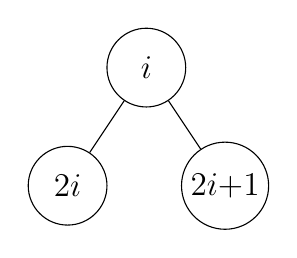
\begin{tikzpicture}[
    level distance=1.5cm,
    sibling distance=2cm,
    every node/.style={circle, draw, minimum size=1cm, inner sep=2pt, font=\large}
]
\node {$i$}
    child { node {$2i$} }
    child { node {$2i{+}1$} };
\end{tikzpicture}
\caption{Array indices in heap}
\label{fig:heap-indices}
\end{figure}

% MAX-HEAPIFY example diagram
\begin{figure}[h]
\centering
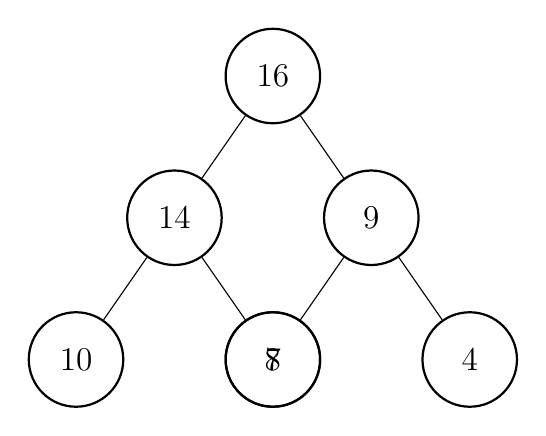
\begin{tikzpicture}[
    level distance=1.8cm,
    sibling distance=2.5cm,
    every node/.style={circle, draw, thick, minimum size=1.2cm, inner sep=2pt, font=\large}
]
\node {16}
    child { node {14}
        child { node {10} }
        child { node {8} }
    }
    child { node {9}
        child { node {7} }
        child { node {4} }
    };
\end{tikzpicture}
\caption{MAX-HEAPIFY example}
\label{fig:max-heapify}
\end{figure}

\textbf{MAX-HEAPIFY Operation:}
\begin{enumerate}
\item Compare root with children
\item If child is larger, swap with largest child
\item Recursively heapify affected subtree
\end{enumerate}

\textbf{BUILD-MAX-HEAP Operation:}
\begin{enumerate}
\item Start from last non-leaf node ($\lfloor n/2 \rfloor$)
\item Apply MAX-HEAPIFY to each node up to root
\end{enumerate}
